%!TEX root = ./Thesis.tex

\chapter{Experimental engineering of qudit states}
\label{chapter:experimental_engineering_qudits}

\tmpHeading{Summary of the work} In this chapter we present an experimental implementation of the state engineering scheme discussed in~\cref{chapter:quantum_walks}, leveraging the \emph{coin space} of a \ac{QW} as an auxiliary degree of freedom to engineer target qudits.
We use for the purpose an experimental apparatus implementing time-dependent \acp{QW} in the polarisation and \ac{OAM} degrees of freedom~\cite{zhang2010implementation,goyal2013implementing,cardano2015quantum}, exploiting the so-called \acp{QP}~\cite{marrucci2006optical} to implement the controlled-shift QW operation.
To benchmark and showcase the potential of the apparatus, we demonstrate the engineering of several classes of states.
The work described in this chapter can be found in~\cite{giordani2019experimental}.

% \tmpHeading{Why \ac{OAM}?} \acf{OAM} allows to encode high-dimensional quantum states in spatially localised photons. Moreover, \acp{QP} intertwine the polarisation and \ac{OAM} degrees of freedom of light, thus allowing more complex dynamics exploiting both types of degrees of freedom.
% With this apparatus, $n$ \ac{QW} steps require $\mathcal O(n)$ optical components -- one \ac{QP} and a few waveplates for each step -- thus making the scheme efficient. Moreover, by having access to fast-enough optical switches and fastly tunable \acp{QP} and waveplates, it is in principle possible to use a single \ac{QP} and waveplate for arbitrary many steps, by having the light pass through the same optical elements multiple times \highlight{(mmmh)}.
% in \emph{light} of the favourable scaling of the number of optical elements with the size of the walk~\cite{reck1994experimental,clements2016optimal}. Moreover, the scheme allows for the full control of the coin operation that is key to the walk implementation of the walk.


% \tmpHeading{What will we conclude from the chapter?}
% The quality of the generated states and the feasibility of the experimental protocol that we have put in place, demonstrate the effectiveness of a hybrid platform for quantum state engineering. Such platform holds together a programmable quantum system, the photonic \ac{QW} in the angular momentum, and classical optimisation algorithms to effectively generate a given target \highlight{???}.

\tmpHeading{Chapter outline}
\Cref{sec:expQWs:OAMintro} gives a brief overview of \ac{OAM} and \acp{VVB}.
In~\cref{sec:expQWs:experimental_apparatus} we describe how the protocol put forward in~\cref{chapter:quantum_walks} is used to experimentally engineer six-dimensional qudits.
We then present and discuss the experimental results in~\cref{sec:expQWs:results}, and give our conclusions and outlook in~\cref{sec:expQWs:conclusions}.


\section{Orbital angular momentum of light}
\label{sec:expQWs:OAMintro}

\tmpHeading{Orbital angular momentum of light}
Electromagnetic fields carry angular momentum \cite{jackson1999classical}.
Classically, the angular momentum density of an electromagnetic field is given, up to constants, by
$\bs M =\bs r\times(\bs E\times \bs B)$. This can be decomposed in an \emph{intrinsic} component, the so-called \emph{spin angular momentum}, and an \emph{extrinsic} one, its \ac{OAM}: $\bs M=\bs S+\bs L$, albeit this decomposition is not gauge invariant, and thus not always sensible~\cite{ohanian1986what,cameron2015azimuthal}.
The spin angular momentum is often understood to be due to an internal degree of freedom of the fields, and is what we usually refer to as the \emph{polarisation} of the field. The OAM is instead a property of the spatial structure of the field.
A first experimental demonstration of transfer of \emph{spin} angular momentum of light to matter was given in~\cite{beth1936mechanical}. A few decades later, Allen and collaborators showed that specific types of laser modes also carry an amount of \emph{orbital} angular momentum, due to the nontrivial phase structure of their transverse beam profile~\cite{allen1992orbital}.
Despite the Poynting vector $\bs E\times \bs B$ always pointing in the propagation direction for transverse beams, and thus $\bs r\times(\bs E\times\bs B)$ being vanishing in such direction, Allen et al. realised that the TEM$_{p\ell q}$ laser modes are in general \emph{not} transverse, but rather have a component in the propagation direction. Because of this, they could show that, for this fields, $\bs M$ has a component in the propagation direction, and thus the beams carry OAM.
Since Allen's groundbreaking work, the OAM of light found several applications in quantum information theory~\cite{allen1999orbital,padgett2004lights,barnett2007orbital,molina-terriza2007twisted,franke-arnold2008advances,yao2011orbital,padgett2017orbital,erhard2017twisted,cozzolino2019highdimensional}.
In particular, OAM of photons has been used for communication protocols~\cite{langford2004measuring}, quantum metrology~\cite{dambrosio2013photonic}, as well as to study quantum correlations~\cite{leach2010quantum,mair2001entanglement,vaziri2002experimental,dada2011experimental,pors2011highdimensional,fickler2012quantum,malik2016multiphoton}.
% that is proportional to $\ell$, which is the quantum number that determines the azimuthal phase profile of the field.
The most common types of helical laser beams carrying OAM are \ac{LG} modes, here denoted with $LG_p^\ell$. These are solutions of the Helmholtz equation in cylindrical coordinates in the paraxial approximation. LG modes are defined by the two quantum numbers $p$ and $\ell$, respectively characterising the radial and azimuthal structure of the mode. A characteristic feature of these beams is their azimuthal phase dependence: $LG_p^\ell\sim e^{i\ell\phi}$ with $\phi$ the azimuthal coordinate in the plane transverse to the propagation direction. LG modes carry an integer amount of OAM.
In~\cref{fig:expQWs:LG_profile_L0P2Z03,fig:expQWs:LG_profile_L1P2Z03} we give two examples of the transverse intensity profile of LG modes with different azimuthal quantum numbers $\ell$.
% ~\cite{mair2001entanglement,kwiat1993highvisibility,howell2004realization,}

\tmpHeading{Coupling OAM with polarisation}
While in vacuum, the spin and orbital components of the angular momentum are conserved, this ceases to be the case in inhomogeneous, anisotropic media. This makes it possible to devise devices which couple spin and OAM of impinging light. One such device is the so-called \acf{QP}~\cite{marrucci2006optical}.
When polarisation and OAM are coupled, we talk of a \acf{VVB}~\cite{cardano2012polarization}.
VVBs find application in multiple fields of classical and quantum optics~\cite{marrucci2011spintoorbital,cozzolino2019highdimensional,cardano2015spin–orbit,rubinsztein-dunlop2016roadmap}.
In the context of quantum information, VVBs have been studied for their peculiar entanglement structure~\cite{dambrosio2016entangled}, quantum communication and cryptography~\cite{vallone2014freespace,wang2015quantum,mirhosseini2015highdimensional,willner2015optical,malik2016multiphoton,sit2017highdimensional,cozzolino2019orbital,cozzolino2019aircore}, quantum walks~\cite{zhang2010implementation,goyal2013implementing,cardano2015quantum}, quantum simulation~\cite{cardano2016statistical,cardano2017detection}, and quantum memories~\cite{parigi2015storage}.

\tmpHeading{Encoding information in VVBs}
Despite their potential, decoding information stored into VVBs remains nontrivial. Efficient \ac{OAM}-demultiplexing requires interferometry~\cite{leach2002measuring,slussarenko2010polarizing,bauer2013nanointerferometric} or spatial filtering~\cite{berkhout2010efficient,bolduc2013exact,malik2014direct},
and these introduce detrimental effects of loss and noise~\cite{qassim2014limitations}.
More generally, the state tomography of such high-dimensional states is always challenging~\cite{paris2004quantum,banaszek2013focus}.
% Moreover, the challenge of performing state tomography of such high-dimensional states can hardly be overestimated
The design and demonstration of reliable techniques to generate and classify \acp{VVB} is thus highly desirable. Previous efforts to find novel platforms to manipulate VVBs~\cite{liu2016generation,ndagano2017creation,cardano2015spin–orbit,rubinsztein-dunlop2016roadmap},
include integrated photonics~\cite{chen2018mapping,cai2012integrated,liu2017direct} and plasmonic metasurfaces~\cite{karimi2014generating,yue2016vector}.


% \begin{figure}[tb]
% 	\centering
% 	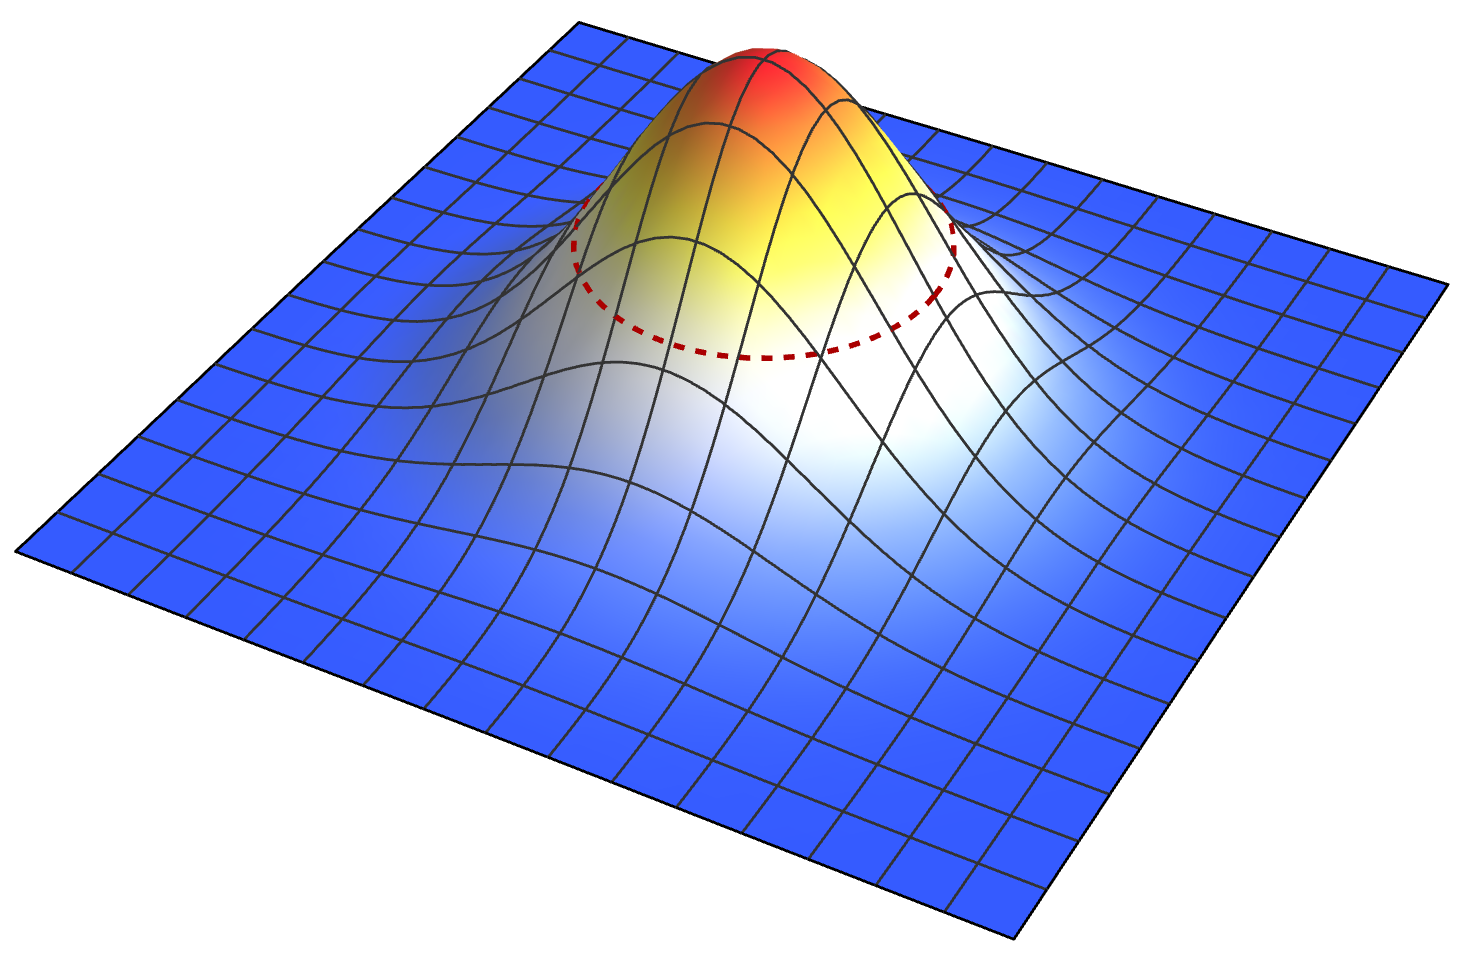
\includegraphics[width=.7\linewidth]{Figures/OAM/GaussianBeam2.png}
% 	\caption{%
% 		Gaussian beam
% 	}
% 	\label{fig:expQWs:gaussian_beam}
% \end{figure}

% \begin{figure}[tb]
% 	\centering
% 	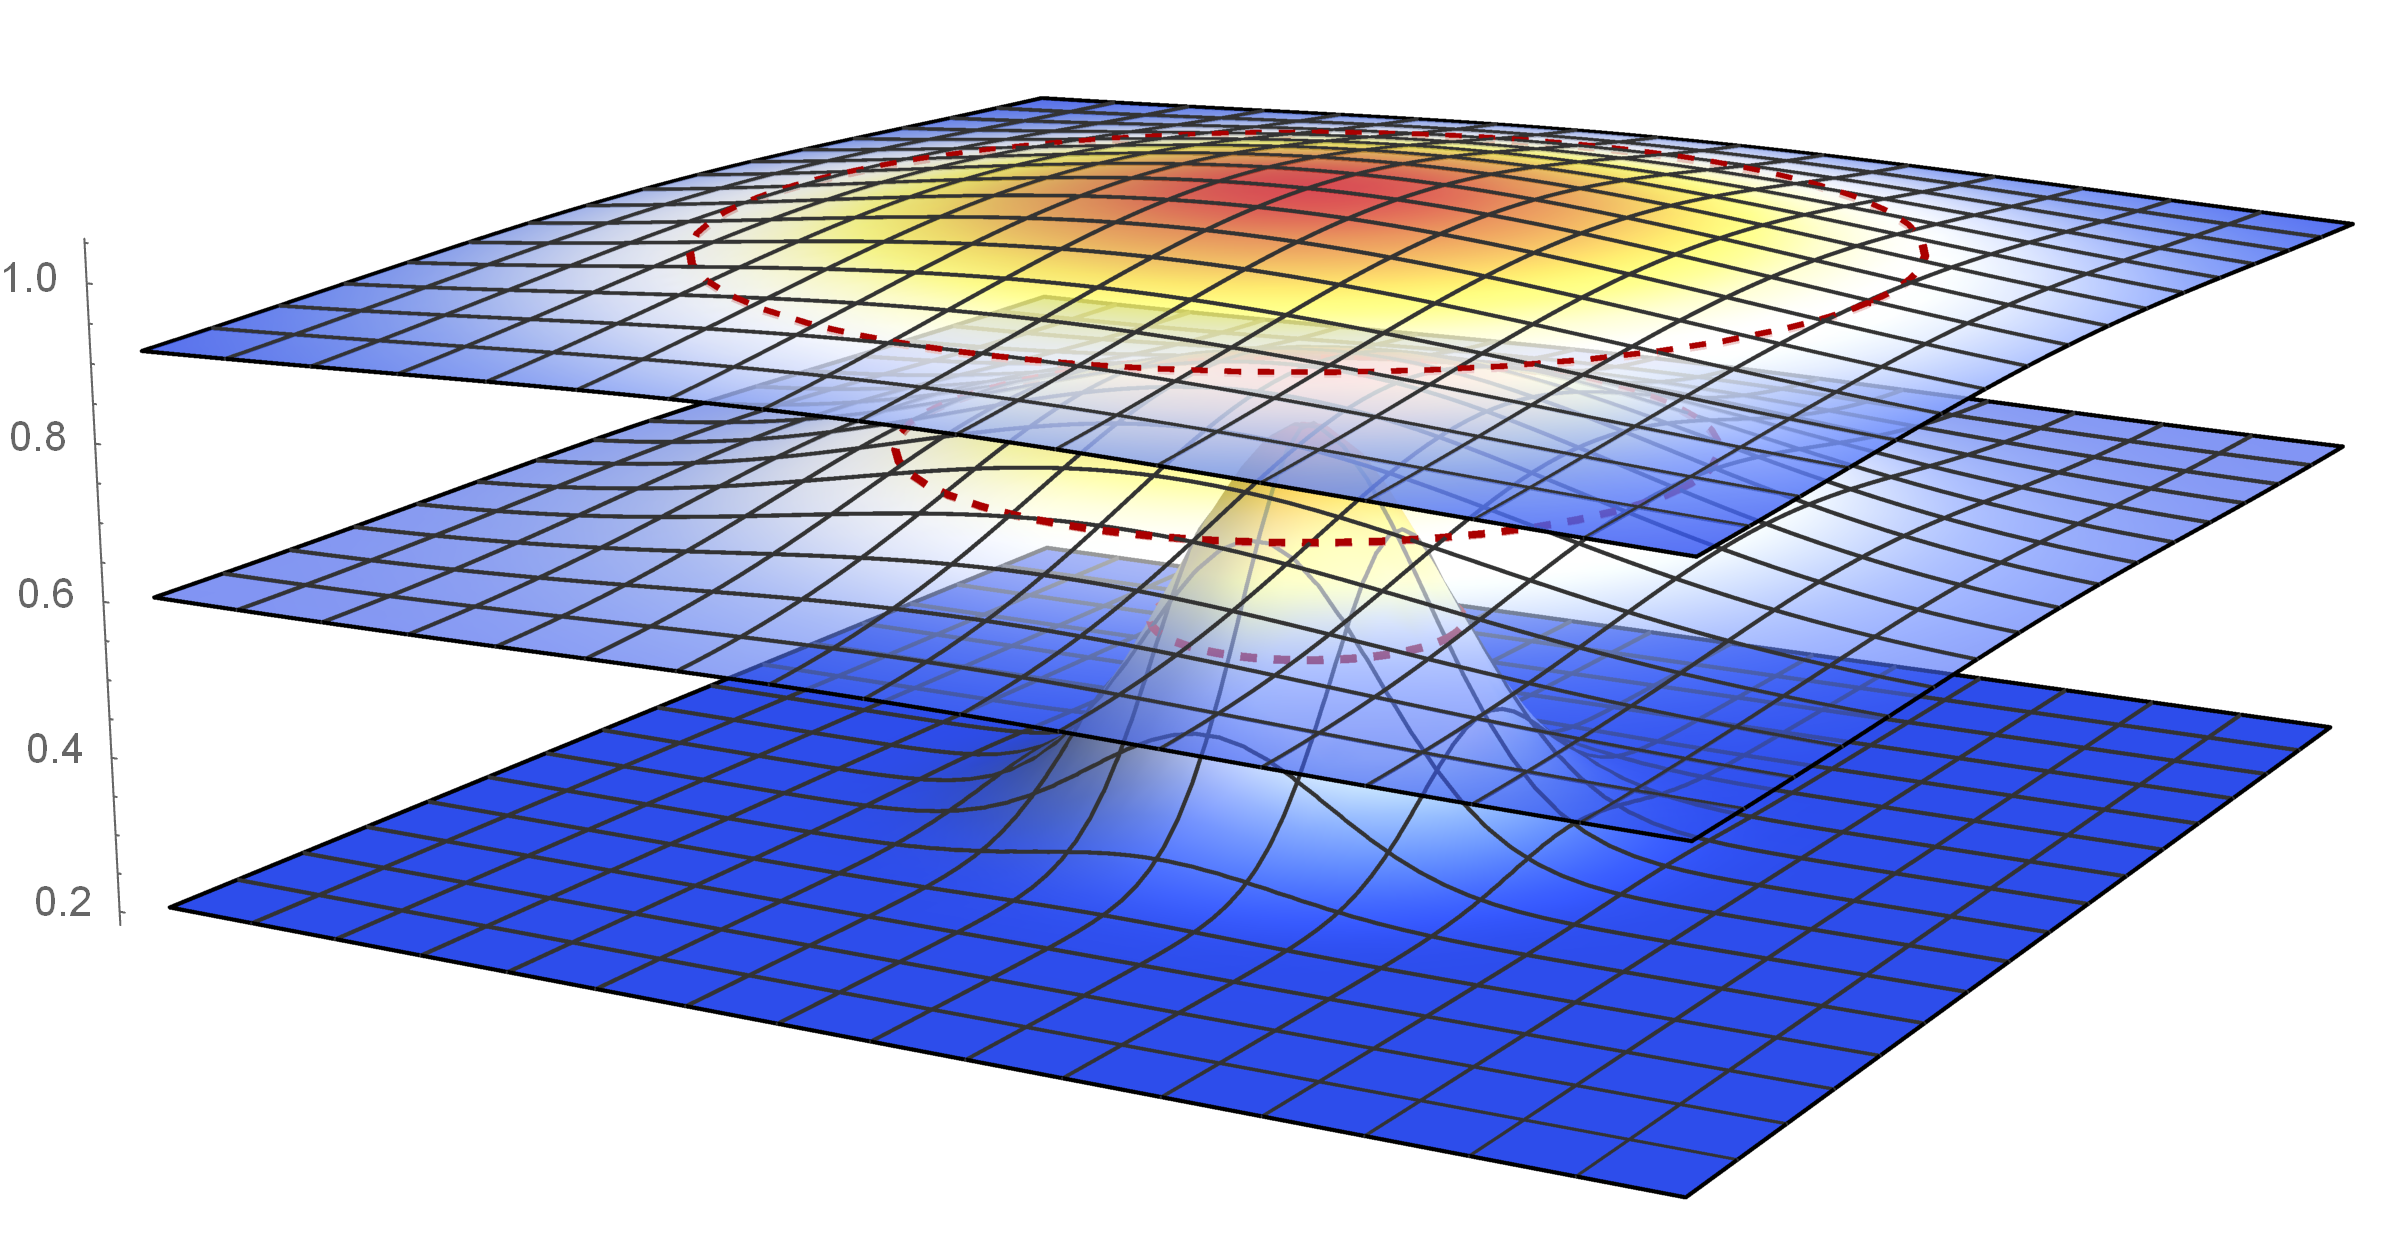
\includegraphics[width=.7\linewidth]{Figures/OAM/GaussianBeamDispersion.png}
% 	\caption{%
% 		Gaussian beam
% 	}
% 	\label{fig:expQWs:gaussian_beam}
% \end{figure}

\begin{figure}
    \centering
    \begin{minipage}{0.45\textwidth}
        \centering
        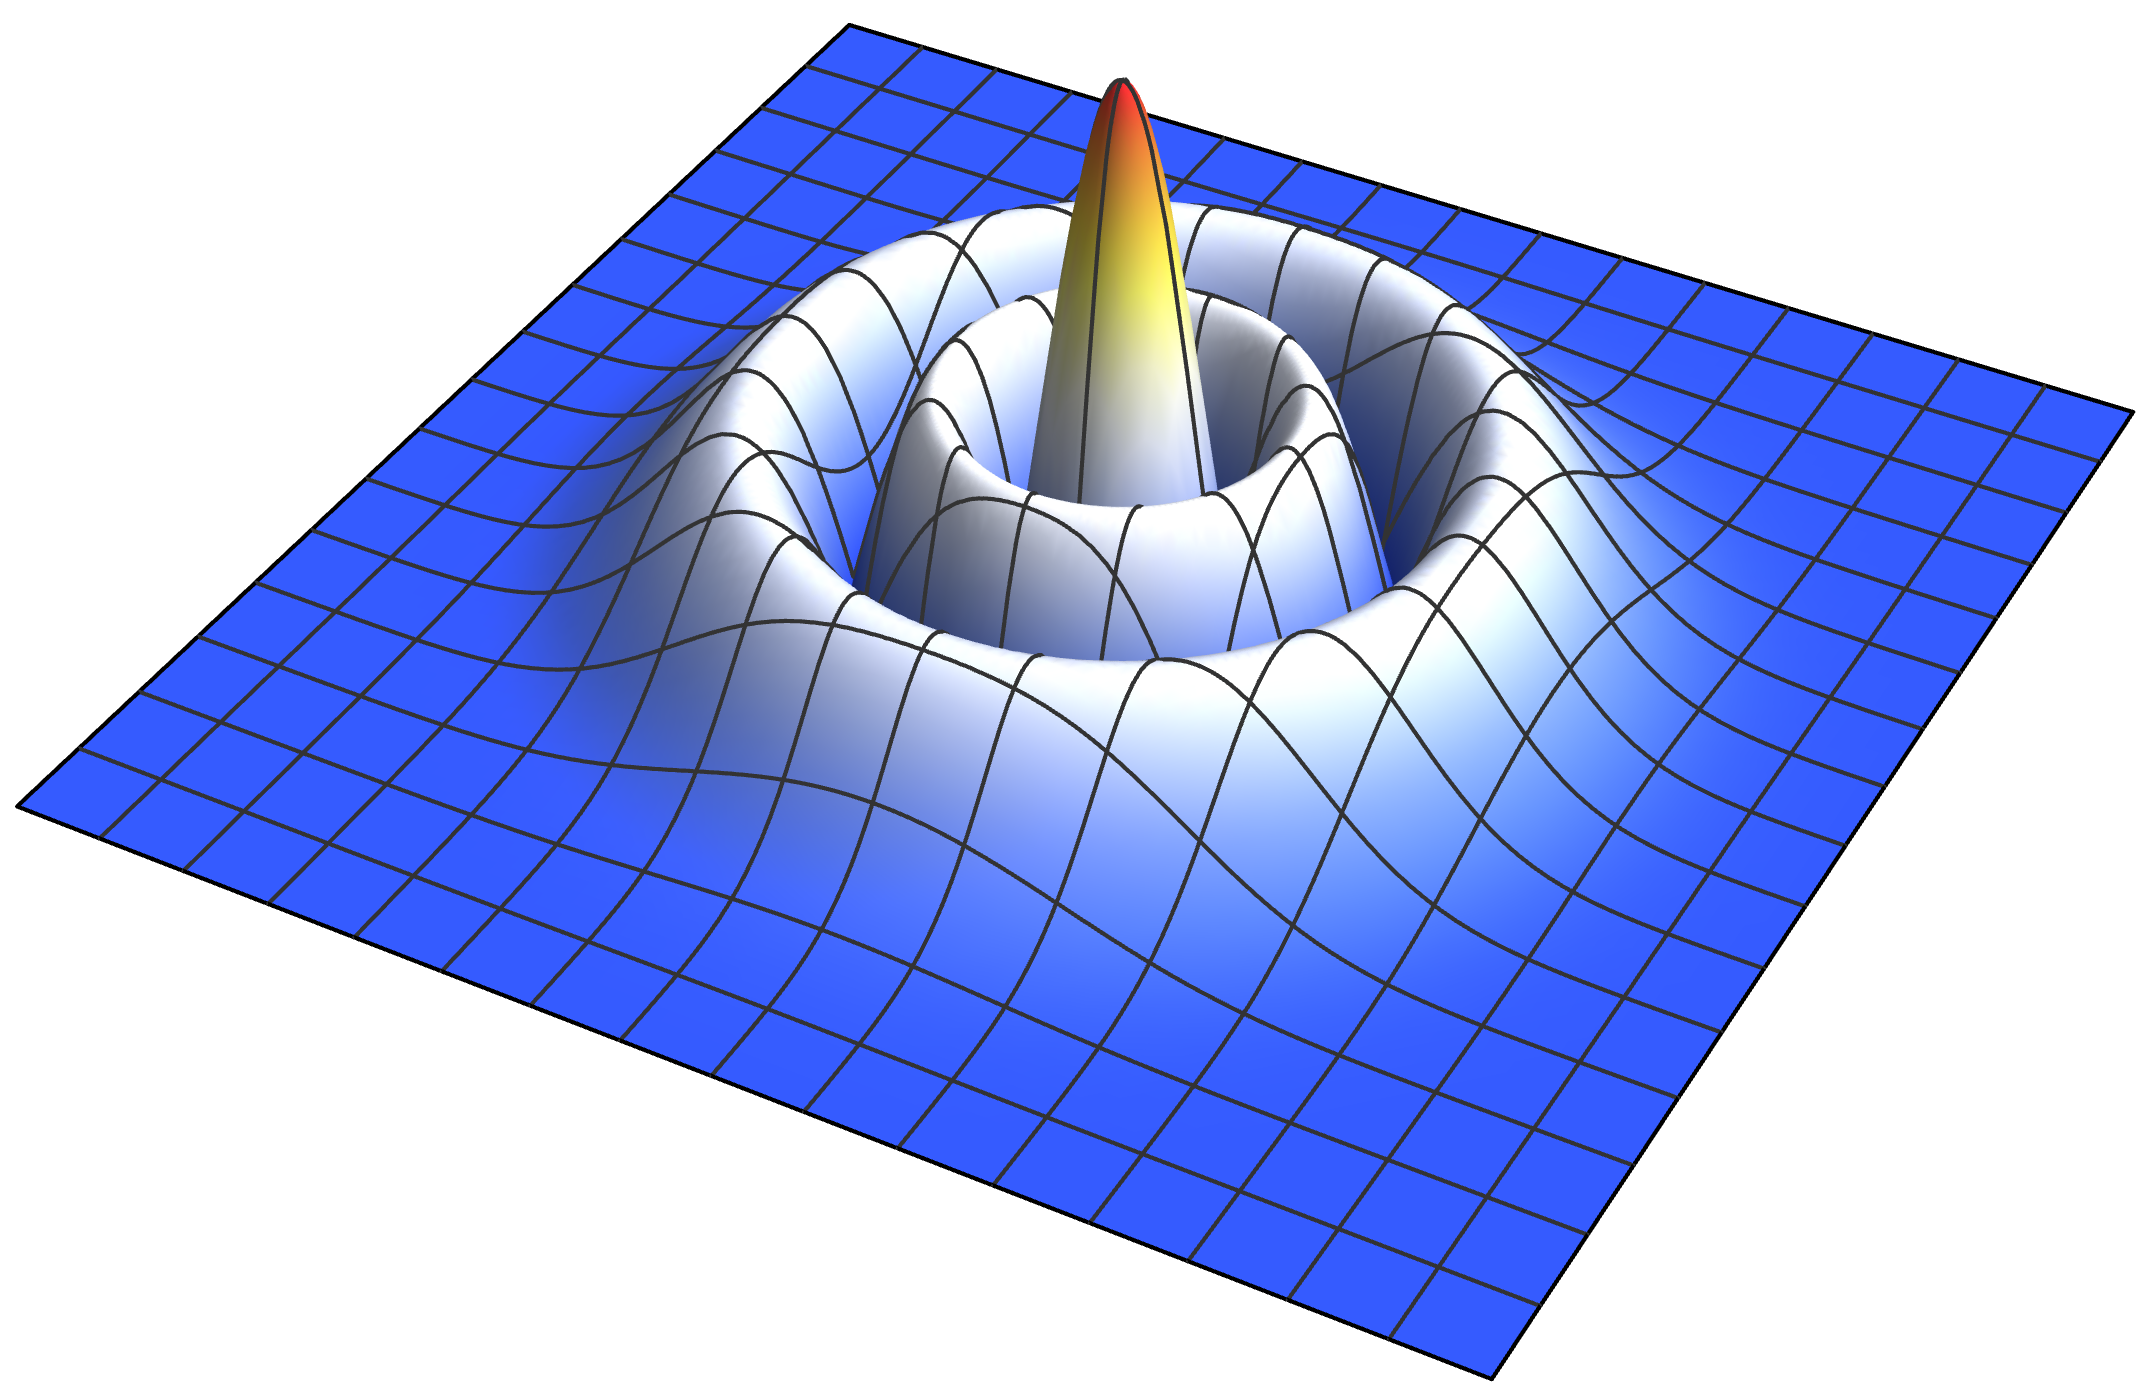
\includegraphics[width=1\textwidth]{Figures/OAM/LGBeamProfile_L0P2Z03.png} % first figure itself
        \caption{
        	Transverse profile of an OAM state with $\ell=0, p=2$.
        	% Transverse profile of an OAM state with $\ell=0, p=2, z=3$.
        }
        \label{fig:expQWs:LG_profile_L0P2Z03}
    \end{minipage}\hfill
    \begin{minipage}{0.45\textwidth}
        \centering
        \vspace{-30pt}%
        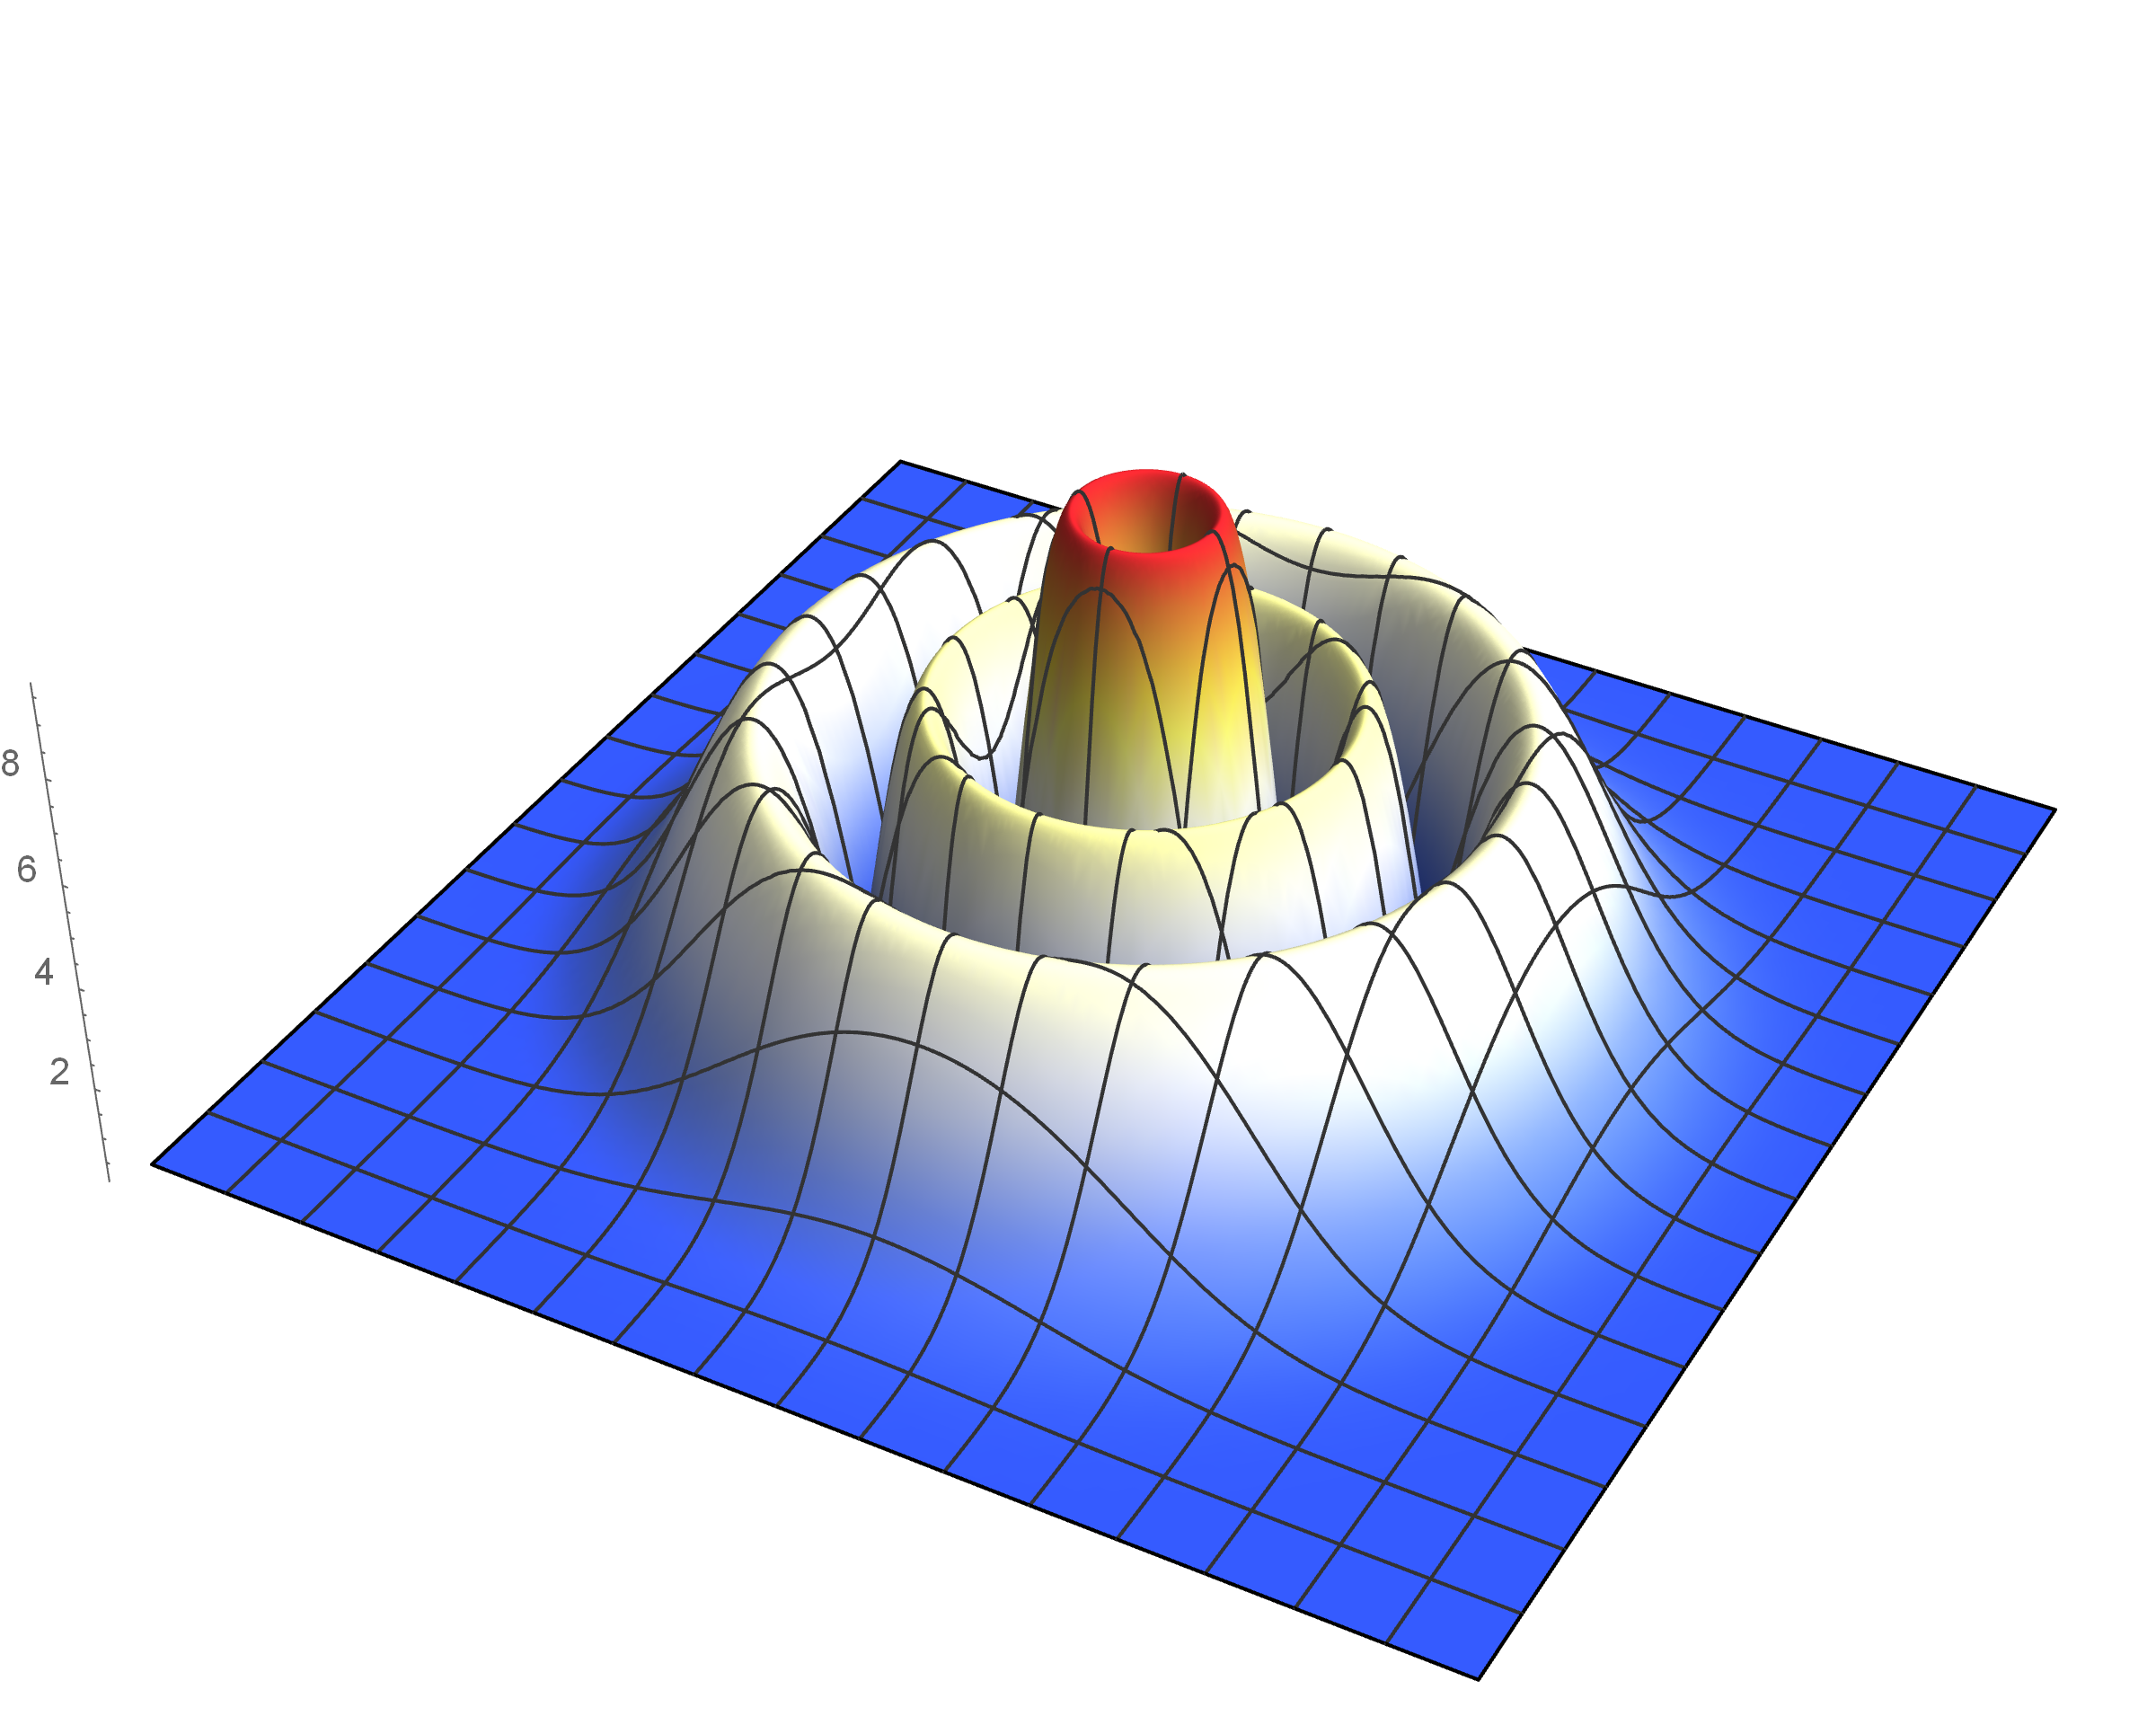
\includegraphics[width=1\textwidth]{Figures/OAM/LGBeamProfile_L1P2Z03.png} % second figure itself
        \caption{
        	Transverse profile of an OAM state with $\ell=1, p=2$.
        	% Transverse profile of an OAM state with $\ell=1, p=2, z=3$.
        }
        \label{fig:expQWs:LG_profile_L1P2Z03}
    \end{minipage}
\end{figure}

% % \FloatBarrier
% \section{State engineering protocol}
% \label{sec:expQWs:engineeringQWs}



\section{State engineering protocol}
\label{sec:expQWs:experimental_apparatus}

% \tmpHeading{What do we do?}
% In~\cref{sec:QWs:reachability_conditions,sec:QWs:focusing_walker_states} we showed that arbitrary qudits can be generated via suitable \ac{QW} dynamics. Here we present an experimental implementation of such protocol, showcasing its practicality in a few relevant scenarios.
% More specifically, we experimentally engineer six-dimensional qudits, focussing on a few physically relevant classes of states: \emph{angular-momentum Schrödinger cat states}, \emph{spin-coherent states}, completely balanced states, and randomly sampled states.

\tmpHeading{Our scheme to implement QWs}
We implement \acp{QW} with $n=5$ steps, using \ac{OAM} as the physical embodiment of the \emph{walker}, and the polarisation as the \emph{coin}. This allows the QW dynamics to take place in a single light beam.
% are encoded in circular-polarisation states $\{|R\rangle, |L\rangle\}$. We dub such degree of freedom as \ac{SAM} to mark the difference with \ac{OAM}.
The experimental setup, shown schematically in~\cref{fig:expQWs:schematics,fig:expQWs:proposal_exp}, is similar to the ones used in~\cite{cardano2015quantum,cardano2016statistical}.
The number of required optical elements scales linearly with the number of QW steps, thus avoiding the nonlinear growth of optical paths intrinsic to interferometric implementations~\cite{zhang2010implementation,goyal2013implementing}.
The coin operations are implemented by suitably arranging polarisation-rotating waveplates~\cite{simon1990minimal}. The shift operator is implemented using \acp{QP}~\cite{marrucci2006optical}. These are birefringent liquid-crystal devices that rise or lower the \ac{OAM} quantum number of impinging light conditionally to its polarisation ~\cite{marrucci2006optical}. More specifically, \acp{QP} act on \ac{OAM} states with azimuthal quantum number $m$ and polarisation $\ket L$ or $\ket R$ as follows:
\begin{equation}
\begin{aligned}
	\ket{L,m} & \xrightarrow{\text{QP}} \cos(\delta/2) \ket{L,m}
				+ i e^{\,-2 i \alpha_0}\, \sin(\delta/2) \ket{R,m+2q}, \\
	\ket{R,m} & \stackrel{\text{QP}}{\longrightarrow} \cos(\delta/2) \ket{R,m}
				+ i e^{-2 i \alpha_0} \sin(\delta/2) \ket{L,m-2q}.
\end{aligned}
\end{equation}
The parameter $q$ is referred to as the \emph{topological charge} of the device.
The phases $\alpha_0$ and $\delta$ are tunable by changing the orientation of the waveplates, and can be chosen so that the QP acts as
\begin{equation}
	\ket{R,m}\xrightarrow{\text{QP}} \ket{L,m-2q}
	\qquad\text{ and }\qquad
	\ket{L,m}\xrightarrow{\text{QP}}\ket{R,m+2q}.
\end{equation}
Single-photon states are generated via a type-II, collinear \ac{SPDC} source, separated with a \ac{PBS}, and then coupled to two \acp{SMF}. One photon acts as the trigger signal, while the other one undergoes the evolution.
% After propagation through the \ac{SMF} and the first \ac{PBS}, the state is $\ket{\psi_0}_{wc}=\ket{0}_w \otimes \ket{+}_c$ with $\ket{+}_c=(\ket{{\uparrow}}_c+\ket{{\downarrow}}_c)/\sqrt2$.
After the $5$ steps, the coin is projected onto $|+\rangle$, following the state engineering protocol outlines in~\cref{sec:QWs:focusing_walker_states}. This is experimentally implemented with a final \ac{PBS}.
To reconstruct the \ac{OAM} states thus generated, the light is coupled into a \ac{SMF} after passing through a \ac{SLM}. This allows to measure arbitrary \ac{OAM} states with high accuracy~\cite{bolduc2013exact,dambrosio2013test}.
The state fidelity between generated and target states is estimated by projecting the \ac{OAM} onto a basis containing the target state.

% Polarisation measurements are performed with waveplates and \acp{PBS}, while the \ac{OAM} is analysed with a \acp{SLM} and \acp{SMF}.
% The \ac{QW} is thus built out of a series of wave plates and QPs. The final state is projected onto OAM basis states using a \ac{SLM}, a \ac{SMF}, and an \ac{APD}.

\begin{figure}[tb]
\centering
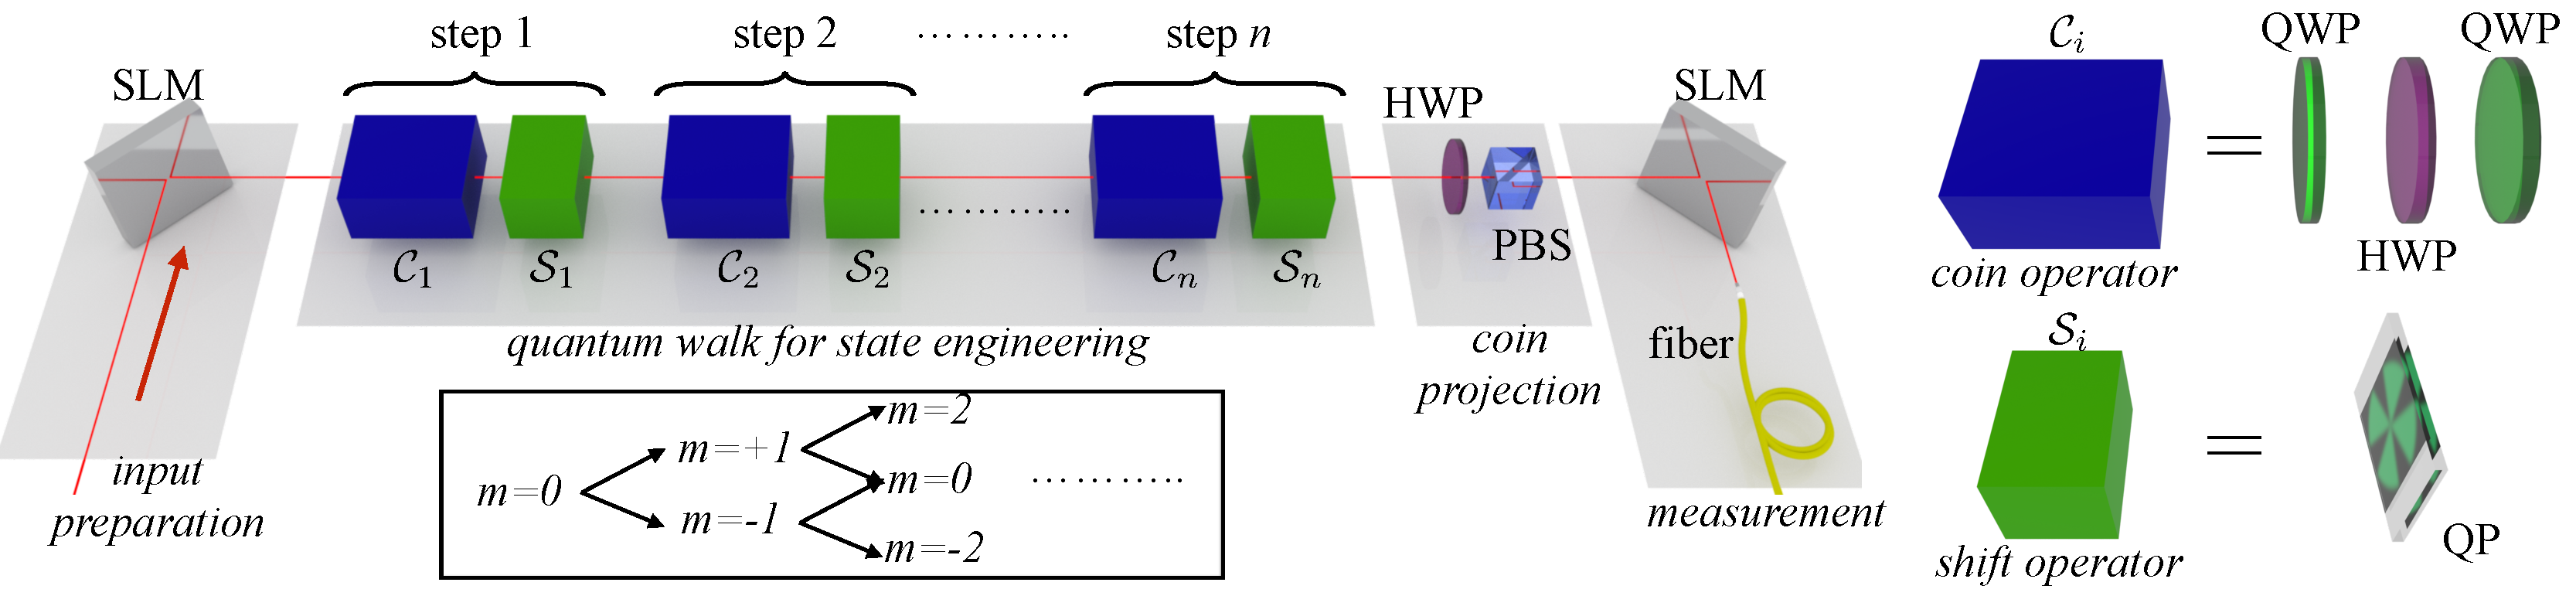
\includegraphics[width=0.99\textwidth]{experimental_apparatus_scheme.pdf}
\caption{
    Pictorial representation of the state engineering protocol.
    Input states are prepared using a \ac{SLM}.
    The coin operations are realised with sequences of \ac{QWP} and \ac{HWP}.
    The shift operations are implemented with \acp{QP}.
    The coin is projected at the end of the walk onto the state $\vert + \rangle$ using a \ac{HWP} and a \ac{PBS}.
    Finally, a \ac{SLM} and a \ac{SMF} are uesd to project the output states onto specific \ac{OAM} states.
}
\label{fig:expQWs:proposal_exp}
\end{figure}

\begin{figure}[tb]
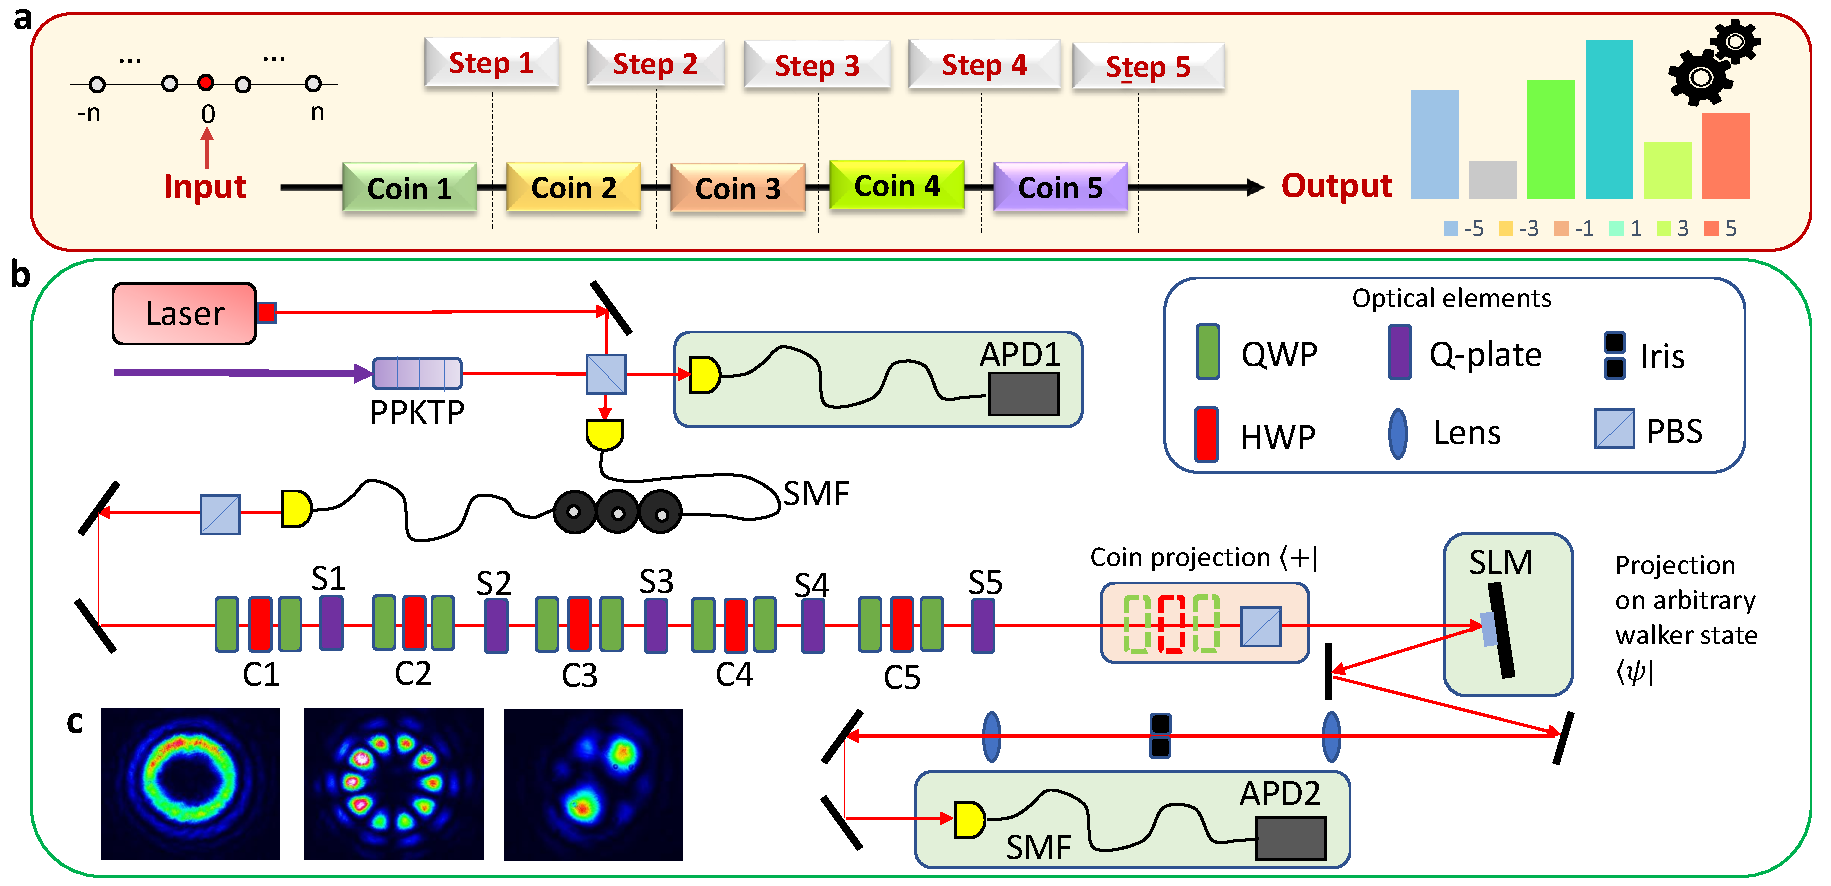
\includegraphics[width=\textwidth]{experimental-QSE-1.pdf}
\caption{
	More detailed representation of the protocol described in~\cref{fig:expQWs:proposal_exp}, focusing on our specific implementation.
	\textbf{(a)} Evolution of the state through to the five different coin operations.
	\textbf{(b)} A single-photon source, composed of a \ac{PPKTP} crystal, generates pairs of photons, which are then coupled in a SMF. One photon acts as trigger while the other one is prepared in the state $\ket{+}\otimes \ket{0}$ through polarisation controllers and a \ac{PBS}. Five sets of \acp{QWP} and \acp{HWP} implement the coin operators at each step. Five \acp{QP} implement the controlled-shift operations.
	The detection stage consists of a \ac{PBS} followed by a \ac{SLM}, a \ac{SMF} and an \ac{APD}.
	\textbf{(c)} Images of \ac{OAM} states detected after the \ac{PBS}. From right to left: \ac{OAM} eigenstate corresponding to $m=5$; balanced superposition of $m=\pm 5$; balanced superposition of all \ac{OAM} components covered by 5-step \ac{QW} $m=\{\pm 5, \pm 3, \pm 1\}$.
}
\label{fig:expQWs:schematics}
\end{figure}

\tmpHeading{Coupling light into the QPs}
Experimental limitations in the maximum achievable number of steps are due to the generation process of \ac{OAM} eigenstates by the \acp{QP}. To prevent coupling between the radial and azimuthal parts of the beam during the propagation in free space, all of the evolution has to happen in the near-field regime~\cite{karimi2009light,cardano2015quantum}. This means that the distance $\ell$ between consecutive \acp{QP} has to be such that $\xi\equiv \ell/z_R \ll 1 $, where $z_R$ is the Rayleigh range.
In our setup, the beam waist $w_0$  ensures a $z_R> \SI{30}{\meter}$ at wavelength $\lambda=\SI{808}{nm}$. Two adjacent \acp{QP} are separated by a distance $\ell \sim \SI{15}{cm}$ (this distance is needed to insert, between the \acp{QP}, the waveplates implementing the coin), such that the condition on $\xi$ is satisfied.  Furthermore, in this regime the Gouy phase can be neglected allowing a good control of the coherence between different \ac{OAM} components, and, consequently, on the output states. However, in the perspective of implementing a higher number of steps, the requirement to have a $z_R$ large at least as the total length $L$ of the platform also implies a large beam waist, thus limiting the maximum amount of steps that can be implemented. An alternative strategy could be to use a loop scheme, where consecutive steps are performed by multiple passes through the same \ac{QP} and waveplates~\cite{goyal2013implementing}. In this alternative setup, a suitable $4f$ lens system is necessary to image the output of the QP to the input of the next step, being such approach equivalent to work in the near-field regime.  
In this combined \ac{OAM}-loop scheme, experimental challenges arise at the measurement stage, that in spin-\ac{OAM} setup involves a \ac{SLM}. When integrating such encoding in a loop-architecture, issues may arise due to their slow response time.


\section{Results}
\label{sec:expQWs:results}

\tmpHeading{Types of generated states}
To demonstrate the flexibility of the protocol, we showcase the generation of a variety of states, including
% \begin{enumerate}
% 	\item Computational basis states;
% 	\item Cat-like states (see~\cref{subsec:expQWs:catstates});
% 	\item \acp{SCS} (see~\cref{subsec:expQWs:SCSs});
% 	\item Completely balanced and randomly sampled states;
% 	\item Fourier basis states.
% \end{enumerate}
computational basis states, completely balanced states, random states, Fourier basis states, cat-like states and \acp{SCS} (see~\cref{subsec:expQWs:catstates}).
% We start by generating the elements of the computational basis corresponding to the eigenstates of the \ac{OAM}: $\{\ket{m} \}=\{\ket{\pm5}, \ket{\pm3},\ket{\pm1} \}$. We then generate superpositions of two computational basis states, and then proceed with more complex states such as spin-coherent states, the elements of the Fourier basis, and lastly random states.
% The quantum state fidelities are calculated projecting onto the elements of an orthonormal basis containing the target state.
\Cref{table:expQWs:summary} contains a summary of the states engineered with the corresponding fidelities and generation probabilities,
while~\cref{table:expQWs:random_states_amps} gives the explicit form of the used random target states.
In~\cref{fig:expQWs:results_cat_states,fig:VVBs:results_SCS_states} we give the experimental results for the generation of cat-like states and \acp{SCS}, respectively.
The fidelity between experimentally synthesised and target states is computed by projecting each state onto an orthonormal basis containing the target one.
% In~\cref{fig:VVBs:results_SCS_states}\textbf{f}, we report the fidelities for all the experimentally engineered states.
% The red area shows the average fidelity and its uncertainty ($\mathcal{F}{=}0.954 \pm 0.001$). Such test provides further evidence of the effectiveness of our engineering strategy.

\tmpHeading{Scaling of projection probabilities}
% As mentioned in~\cref{sec:QWs:focusing_walker_states}, multiple \ac{QW} dynamics can, after projection of the coin, lead to the same target state.
% These different solutions will in general correspond to different projection probabilities.
% To find the coin operators leading to each target state we used the numerical optimisation method presented in~\cref{sec:QWs:numerical_fid_max}.
% To assess the average scaling on the projection probability, we simulated QWs of up to $20$ steps using the algorithm of~\cref{sec:QWs:numerical_fid_max} to find coin operations generating different target states. We found the projection probabilities to have a roughly linear scaling, and remain $\ge 15\%$ for up to $20$ steps of our protocol, as shown in~\cref{fig:expQWs:avgProbabilitiesVsStepNumber}.
In~\cref{fig:expQWs:avgProbabilitiesVsStepNumber} we give the \textit{average} projection probability as a function of the number of steps. These are calculated by averaging the projection probabilities obtained by running the optimisation algorithm given in~\cref{sec:QWs:numerical_fid_max} over many uniformly sampled random states, for various numbers of steps. We find the average projection probability to decrease roughly linearly with the number of steps. Assuming such linear behaviour to hold for more steps, the average projection probability would drop to $\sim 0.1$ at around $25$ steps, remaining $\ge 0.15$ for up to $20$ steps.
We note that this likely underestimates the actual probabilities. Indeed, as already mentioned, this optimisation method finds only one among many solutions for a given target, and thus generally not the optimal one in terms of projection probability. Moreover, increasing the number of steps also increases the number of ways in which a state can be generated, meaning that we can expect the underestimation to be more significant for larger numbers of step.
Further evidence suggesting that this method underestimates the real average probabilities is obtained by computing the full set of solutions and taking the optimal one, which can be done for up to five steps. Indeed, as shown in~\cref{sec:QWs:numerical_fid_max}, with this method we find the real optimal average probabilities for three, four, and five steps to be consistently $\sim 0.33$, with no detectable decreasing behaviour.

\begin{table}[tbh]
\centering%\footnotesize
\fontsize{10pt}{10pt}\selectfont
\begin{tabular}{lcc|lcc}
\toprule
Target State & Probability  & Fidelity & Target State & Probability  & Fidelity \\
\midrule
 $\quad\ket{-5}$ & $0.5$  & $0.981 \pm 0.007\quad$ & $\quad\ket{\on{QFT}_1}$ & $0.14$ & $0.969\pm 0.007$\\
 $\quad\ket{-3}$ & $0.5$ & $0.982 \pm 0.007\quad$ & $\quad\ket{\on{QFT}_2}$ & $0.17$ & $0.923\pm 0.022$ \\
 $\quad\ket{-1}$ & $0.5$ & $0.960 \pm 0.007\quad$ & $\quad\ket{\on{QFT}_3}$ & $0.17$ & $0.911\pm 0.011$\\ 
 $\quad\ket{1}$ & $0.5$ & $0.995 \pm 0.007\quad$ & $\quad\ket{\on{QFT}_4}$&$0.17$ &  $0.980\pm 0.011$ \\
 $\quad\ket{3}$ & $0.5$ & $0.975 \pm 0.007\quad$ & $\quad\ket{\on{QFT}_5 }$& $0.17$& $0.936\pm 0.011$ \\
 $\quad\ket{5}$ & $0.5$ & $0.994 \pm 0.001\quad$ & $\quad\ket{\on{QFT}_6} $& $0.17$ & $0.945\pm 0.007$ \\
 $\quad\frac{1}{\sqrt{2}}\left(\ket{-5}+\ket{5} \right)$ & $0.5$  & $0.995 \pm 0.001\quad$ &$\quad\ket{r_1}$ & 0.22& $0.911\pm0.011$\\
 $\quad\frac{1}{\sqrt{2}}\left(\ket{-5}-\ket{5}\right)$ & $0.5$ & $0.947 \pm 0.002\quad$ &$\quad\ket{r_2}$  & 0.16 & $0.923 \pm 0.012$\\
 $\quad\frac{1}{\sqrt{2}}\left(\ket{-5}+i\ket{5}\right)$ & $0.5$ & $0.969 \pm 0.002\quad$ &$\quad\ket{r_3}$  & 0.17 & $0.941 \pm 0.004$\\ 
  $\quad\frac{1}{\sqrt{2}}\left(\ket{-5}-i\ket{5}\right)$ & $0.5$ & $0.936 \pm 0.003\quad$&$\quad\ket{r_4} $& 0.14 &$0.947 \pm 0.015$  \\
 %$\frac{1}{\sqrt{2}}\left(\ket{-3}+\ket{3}\right)$ & $0.5$ & $0.912 \pm 0.004$ \\
 $\quad\ket{S_1}=\ket{5/2,\pi /2,0}$ & $0.15$ & $0.970 \pm 0.002\quad$ &$\quad\ket{r_5}$ & 0.19 & $0.950\pm0.005$  \\
 $\quad\ket{S_2}=\ket{5/2,-\pi /2,0}$ & $0.15$ & $0.961 \pm 0.003\quad$ &$\quad\ket{c_1}$ &0.16 & $0.956\pm0.004$ \\
 $\quad\frac{1}{\sqrt{2}}\left(\ket{S_1}+\ket{S_2}\right)$ & $0.15$ & $0.932 \pm 0.004\quad$&$\quad\ket{c_2}$ & 0.29 &$0.935 \pm 0.006$  \\
 $\quad\frac{1}{\sqrt{2}}\left(\ket{S_1}-\ket{S_2}\right)$ & $0.15$ & $0.942 \pm 0.004\quad$& $\quad\ket{c_3}$& 0.17 & $0.925\pm 0.008$ \\
$\quad\frac{1}{\sqrt{2}}\left(\ket{S_1}-i\ket{S_2}\right)$ & $0.23$ & $0.974 \pm 0.003\quad$&$\quad\ket{c_4}$ & 0.16 & $0.944\pm0.008$\\
$\quad\frac{1}{\sqrt{2}}\left(\ket{S_1}+i\ket{S_2}\right)$ & $0.23$ & $0.964 \pm 0.004\quad$& $\quad\ket{c_5}$ & 0.28 & $0.946\pm0.004$\\
\bottomrule
\end{tabular}
\caption{%
	Generated states with associated projection probabilities and fidelities.
	Left column: computational basis states $\ket k$ with $k\in\{-5,-3,-1,1,3,5\}$, cat-like states, and \acp{SCS} $\ket{S_i}$ and their superpositions.
	Right column: Fourier basis states $\ket{\on{QFT}_k}$, random real states $\ket{r_k}$, and random complex states $\ket{c_k}$.
	The Fourier basis states are defined as $\ket{\on{QFT}_k}=\frac{1}{\sqrt{6}}\sum_{j=1}^{6}e^{\frac{ i \pi jk }{3}}\ket{j}$.
}
\label{table:expQWs:summary}
\end{table}

\begin{table}[tbh]
\centering\footnotesize
\begin{tabular}{cc}
\toprule
State & Amplitudes \\
\midrule
$\qquad\ket{r_1}\qquad$& $\left( 0.51, 0.27, 0.13, 0.10, 0.29, 0.75\right)$\\
$\qquad\ket{r_2}\qquad$& $\left( 0.19, 0.40, 0.04, 0.53, 0.37, 0.62\right)$\\
$\qquad\ket{r_3}\qquad$&$\left( 0.50, 0.74, 0.40, 0.16, 0.10, 0.006\right)$ \\
$\qquad\ket{r_4}\qquad$& $\left( 0.50, 0.47, 0.55, 0.31, 0.36, 0.04\right)$ \\
$\qquad\ket{r_5}\qquad$& $\left( 0.24, 0.12, 0.72, 0.16, 0.54, 0.30\right)$ \\
$\qquad\ket{c_1}\qquad$& $\left( 0.04+0.35i, 0.34+0.41i, 0.10+0.42i, 0.18-0.26i, 0.11-0.11i, -0.47+0.22i\right)$  \\
$\qquad\ket{c_2}\qquad$& $\left( 0.19-0.33i, -0.43+0.30i, -0.18-0.02i, -0.37+0.42i, -0.12-0.10i, 0.23+0.38i\right)$\\
$\qquad\ket{c_3}\qquad$& $\left( -0.19-0.30i, -0.02+0.39i, 0.30-0.15i, 0.25-0.22i, -0.13+0.42i, 0.24+0.48i\right)$\\
$\qquad\ket{c_4}\qquad$& $\left( 0.06+0.07i, 0.30-0.37i, -0.23+0.08i, 0.11-0.13i, -0.22+0.57i, 0.07-0.54i\right)$\\
$\qquad\ket{c_5}\qquad$& $\left( 0.07+0.14i, 0.48-0.34i, -0.41-0.18i, -0.41-0.09i, -0.10+0.32i, 0.32+0.18i\right)$\\
\bottomrule
\end{tabular}
\caption{
	Amplitudes of random target states.
	The real states $\ket{r_k}$ have been sampled uniformly in the range $\left[0,1\right]$ and then normalised. In the case of complex states we have sampled the real and imaginary part separately in the range $\left[-0.5,0.5\right]$.
}
\label{table:expQWs:random_states_amps}
\end{table}

\subsection{Cat-like and spin-coherent states}
\label{subsec:expQWs:catstates}
% \subsection{Spin-coherent states}
% \label{subsec:expQWs:SCSs}

\tmpHeading{What do we mean by ``cat-like states''}
\emph{Schrödinger's cat states} are quantum superpositions of macroscopically distinct states~\cite{yurke1986generating,bužek1995quantum}.
They play an important role in the foundations of quantum mechanics~\cite{schrodinger1935gegenwartige} and their generation is at the core of various quantum engineering protocols~\cite{brune1992manipulation, monroe1996schrodinger,agarwal1997atomic, zhang2016creating}.
In the context of QWs, we define \emph{cat-like states} as coherent superpositions of two extremal sites of the walker, that is, in our case, states of the form $\alpha\ket{5}+\beta\ket{-5}$~\cite{zhang2016creating}. The isomorphism between \ac{OAM} with an angular momentum of quantum number $n/2$ allows to put in correspondence the position states $\ket{\pm 5}$ of the walker with angular momentum states with minimum and maximum projections onto the quantisation axis $\ket{\pm 5/2}$ (for simplicity of notation, we will use position states only here). Such isomorphism makes a coherent superposition state such as $(\ket{5}+e^{i\varphi}\ket{-5})/\sqrt{2}$ (with $\varphi$ a suitable phase) into a faithful angular momentum SCS~\cite{militello2006distilling}. 
% Experimental generation of cat-like states has been previously reported in atomic systems~\cite{leibfried2005creation}.


\begin{figure}[tb]
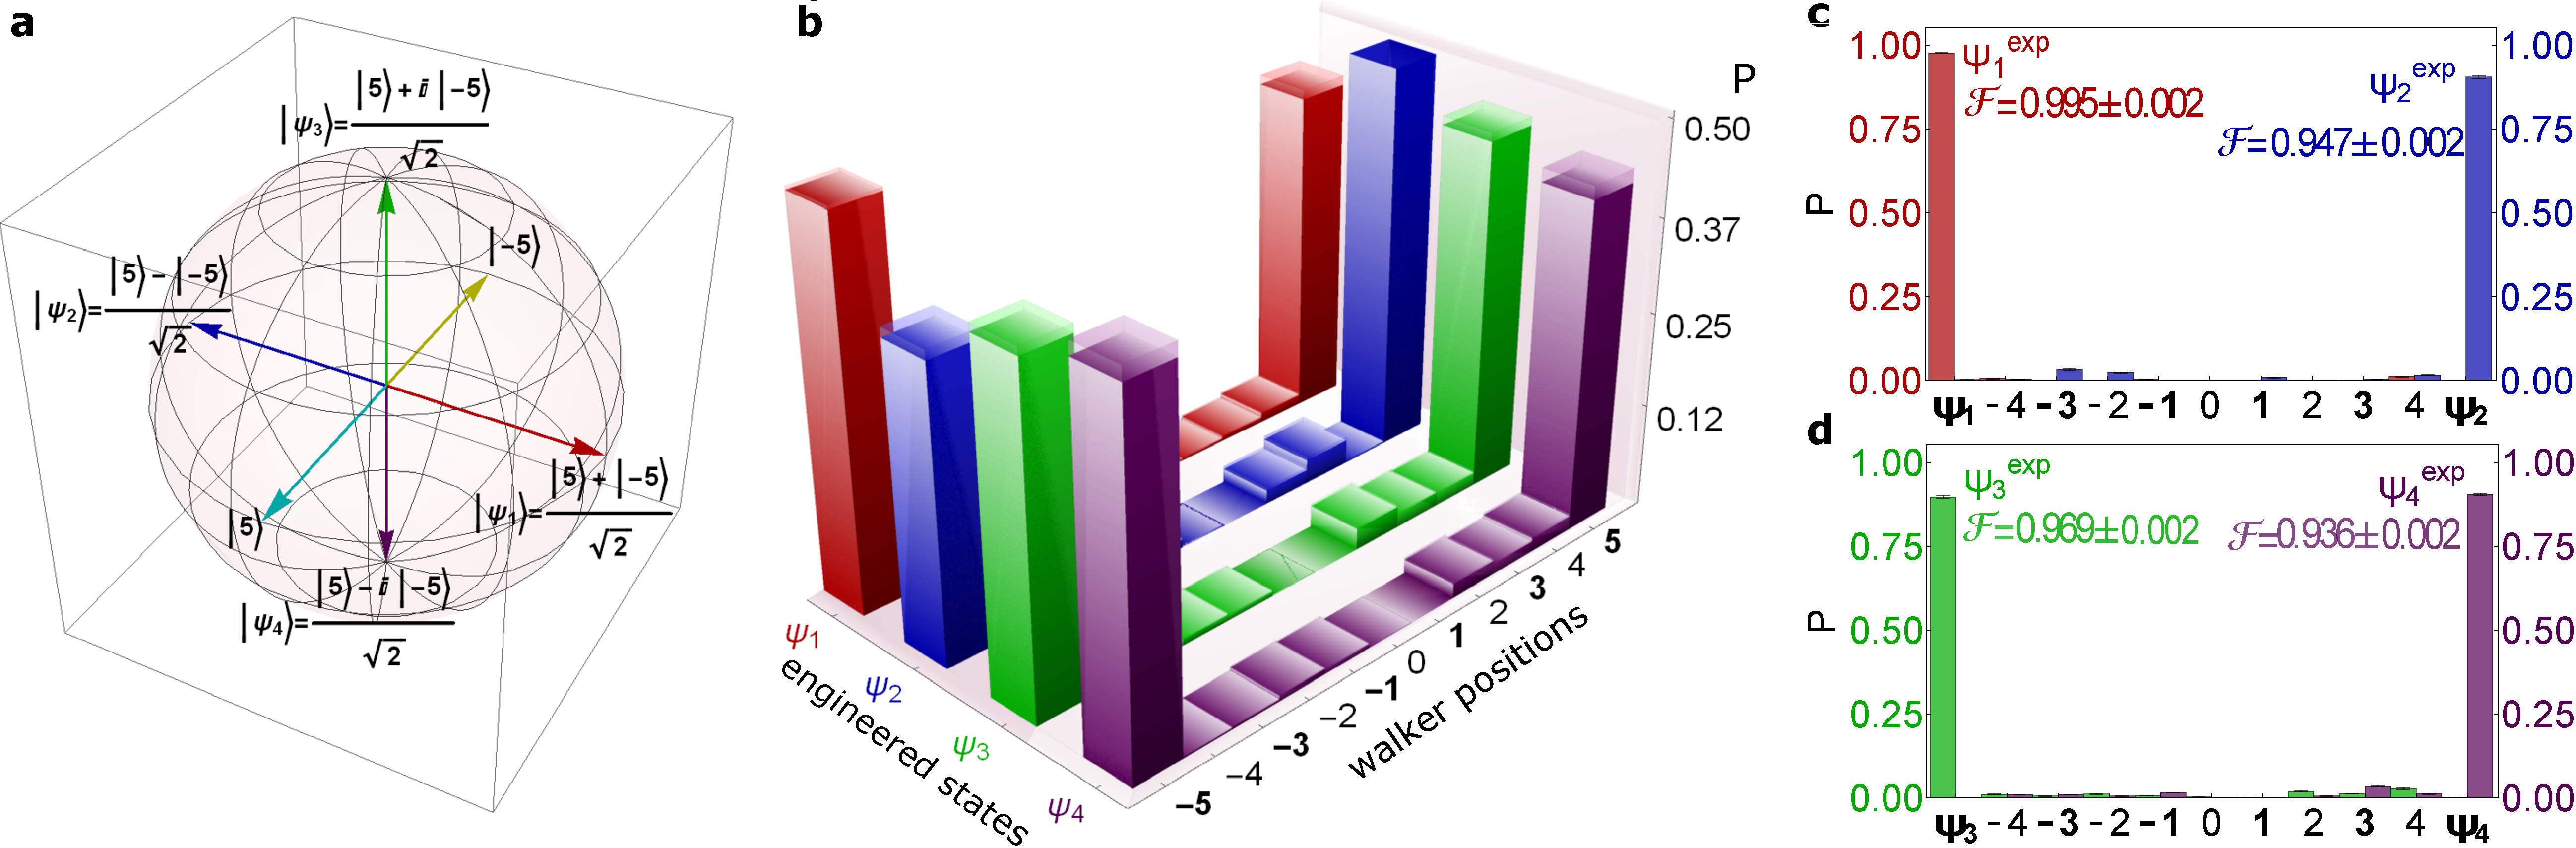
\includegraphics[width=\textwidth]{experimental-QSE-2.pdf}
\caption{
	Experimental results for the angular momentum cat states engineering.
	\textbf{(a)} Bloch sphere representation of the four target states, corresponding to the superposition of $\ket{\pm 5}$. These correspond to \ac{OAM} states with maximum and minimum projection of the angular momentum.
	 % along the quantisation axis.
	\textbf{(b)}
	Populations of different \ac{OAM} modes after $5$-step, when the initial state is one of those used in \textbf{(a)}. Odd-numbered positions are the only ones involved in the state engineering protocol. The small non-zero populations of even-$m$ modes are due to imperfections at generation and detection stages. The error bars associated with experimental populations are shown by the transparent areas on top of each histogram.
	\textbf{(c)-(d)} Probabilities $P_i=\langle B^{(j)}_i\vert\rho_\text{exp}\vert B^{(j)}_i\rangle~(j=1,2)$ of finding the experimental state $\rho_\text{exp}$ in one of the elements of the basis $B^{(j)}=\{\ket{\psi_p},\ket{\psi_{p+1}},\ket{\pm4},\ket{\pm3},\ket{\pm2},\ket{\pm1},\ket{0}\}$ with $p=1$ for $j=1$ and $p=3$ for $j=2$. All the error bars are due to Poissonian uncertainties, propagated through Monte Carlo methods.
	% The state fidelities ${\cal F}$ are calculated as described in the text.
}
\label{fig:expQWs:results_cat_states}
\end{figure}

\begin{figure}[tb]
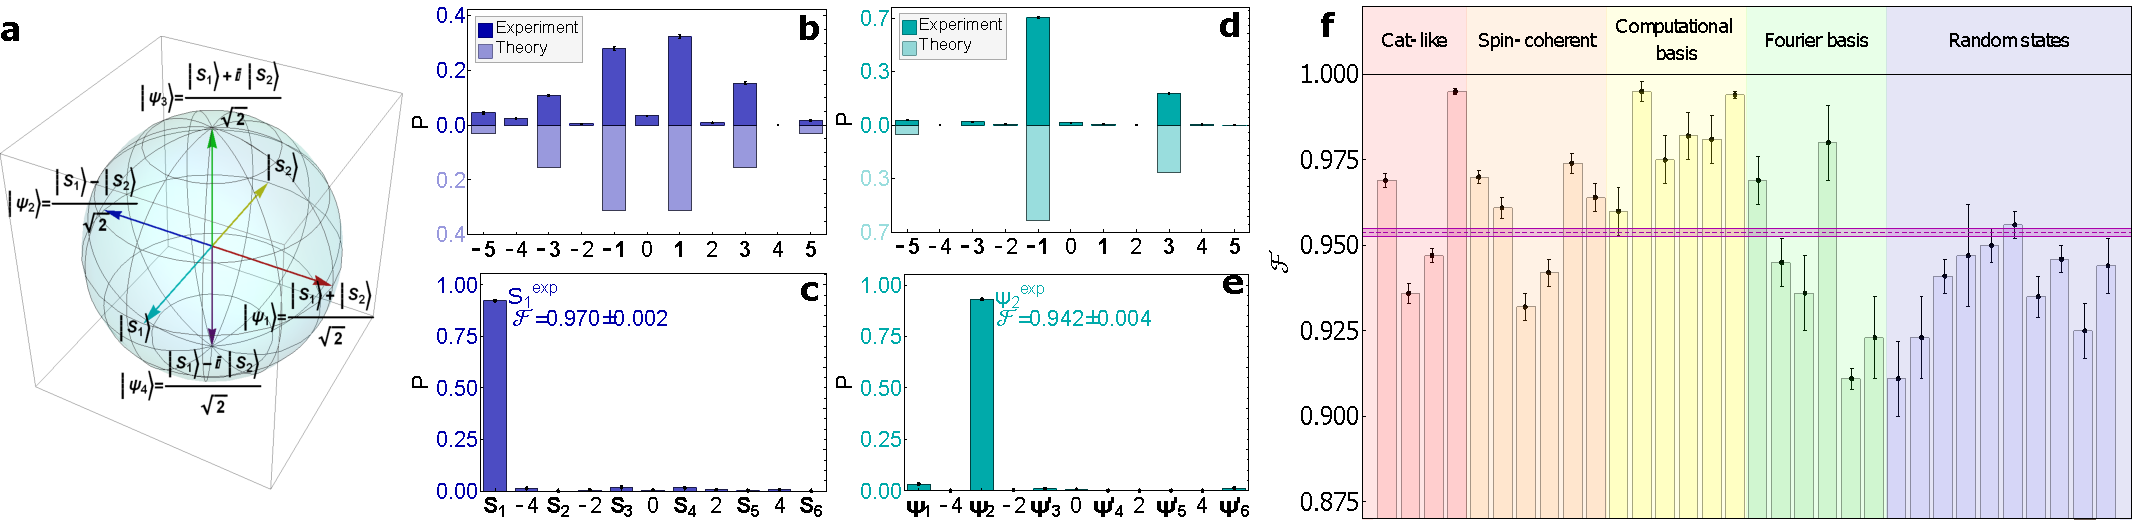
\includegraphics[width=\textwidth]{experimental-QSE-3.pdf}
\caption{
	Experimental results for the engineering of \acp{SCS} and their coherent superposition.
	\textbf{(a)} Bloch-sphere representation of different superpositions of the \acp{SCS} $\ket{S_1}, \ket{S_2}$.
	\textbf{(b)} Probability distributions of projection of $\ket{S_1}$ onto the computational basis.
	% As previously explained, we also consider the contribution of even \ac{OAM} components.
	\textbf{(c)} Probability distribution corresponding to a basis containing $\ket{S_1}$. The fidelity is $\calF\simeq 0.97$.
	The elements of the chosen orthonormal basis, $\{S_i\}_i$ with $i=1 ...6$, are the eigenstates of $\hat{S}_x$ for a particle with spin $s=5/2$.
	% that are in turn all spin-coherent states.
	\textbf{(d)} Probability distribution for $\ket{\psi_2}=\frac{1}{\sqrt{2}}\left(\ket{S_1}- \ket{S_2} \right)$. Only the components $\ket{-5}, \ket{-1}, \ket3$, are expected to have non-zero probabilities.
	\textbf{(e)} Probability distribution with respect to a basis containing the target state $\ket{\psi_2}$.
	The fidelity is $\calF\simeq 0.94$.
	\textbf{(f)} Summary of quantum state fidelities for the $32$ states generated in the experiment. The average fidelity, $\bar{\calF}=0.954\pm 0.001$, is marked by the magenta line.
}
\label{fig:VVBs:results_SCS_states}
\end{figure}

\begin{figure}[tb]
    \centering
    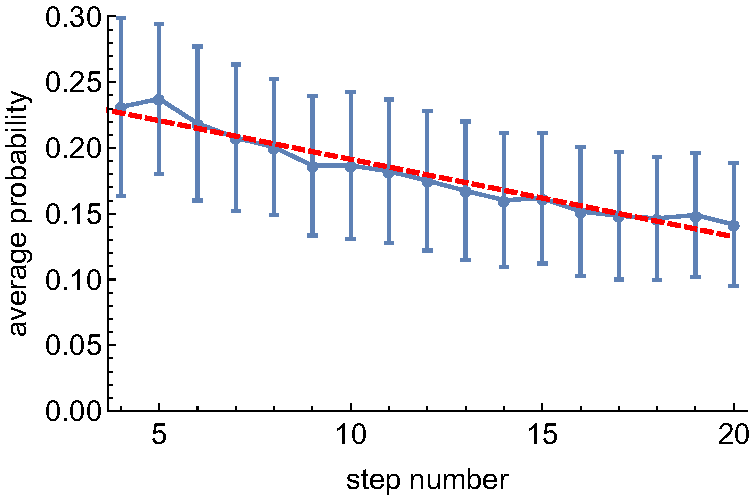
\includegraphics[width=0.8\linewidth]{experimentalQSE-averagesAndVariances_rerundata_manysteps.pdf}
    \caption{
    	Average projection probability obtained for randomly sampled target states with different numbers of steps. Each point corresponds to an average over a sample of $2000$ uniformly sampled random target states of the given dimension. For each target, an optimisation algorithm is used to find a solution producing it, as discussed in~\cref{sec:QWs:numerical_fid_max}. The error bars represent the standard deviation associated with each point. The red dashed line is a linear fit. It should be noted that, as discussed in~\cref{sec:QWs:numerical_fid_max}, this data provides only a lower bound to the real average probabilities.%
    }
    \label{fig:expQWs:avgProbabilitiesVsStepNumber}
\end{figure}

% The second class of states that we consider are \emph{spin-coherent states}~\cite{ulyanov1999spin}, which are the spin-like counterpart of \emph{coherent states} of a quantum harmonic oscillator.

\tmpHeading{What are SCSs?}
\acfp{SCS} are the counterparts of coherent states of the harmonic oscillator for a particle with spin $s$~\cite{radcliffe1971some,arecchi1972atomic,agarwal1997atomic,markham2003classicality,chryssomalakos2018geometry}. They are the eigenstates, with eigenvalue $s$, of $S_{\theta,\phi}$, the component of the total spin-momentum operator along the direction identified by the spherical angles $(\theta, \phi)$~\cite{arecchi1972atomic,agarwal1997atomic,ulyanov1999spin,lee2015visualizing}.
A decomposition of such states over the $\{\ket{m}\}$ basis of the projected spin along the $z$-direction, $S_z$, reads
\begin{equation}
\begin{aligned}
	\ket{s,\theta,\phi} &=
		\sum_{m=-s}^{s}
		\sqrt{\frac{(2s)!}{(s+m)!(s-m)!}} e^{-i\phi m} C_\theta^{s+m} S_\theta^{s-m}\ket{m},
\end{aligned}
\label{spin_coherent1}
\end{equation}
with $C_\theta\equiv\sqrt{1-S^2_\theta}=\cos(\theta/2)$. \acp{SCS} have numerous applications in condensed matter physics, in particular for quasi-exactly solvable models, for the Wigner-Kirkwood expansion and in quantum correction to energy quantisation rules~\cite{ulyanov1999spin}. At a more foundational level, they can be used to generate Schrödinger cat states~~\cite{agarwal1997atomic}. 

\tmpHeading{Properties of SCSs}
Although \acp{SCS} are in general not orthogonal, they form a convenient basis. Moreover, as two \acp{SCS} pointing in opposite azimuthal directions are orthogonal for $\theta\sim\pi/2$, by restricting the attention to $\{\ket{s,\pi/2,\phi},\ket{s,-\pi/2,\phi}\}$ we would be dealing with an orthonormal basis, which we can use to construct the analogous of a Bloch ball for a two-level system (cf.~\cref{fig:VVBs:results_SCS_states}\textbf{a}). We have thus engineered $\ket{S_1}\equiv\ket{5/2,\pi/2,0}$ and $\ket{S_2}\equiv\ket{5/2,-\pi/2,0}$, and considered the experimental synthesis of balanced coherent superpositions of such states.
Furthermore, $S_1$ and $S_2$ are also eigenstates of the $\hat{S}_x$ operator. In~\cref{fig:VVBs:results_SCS_states}\textbf{b-c} the state $S_1$ is projected firstly on the computational basis, the eigenstates of $\hat{S_z}$, and then on the basis $\{S_i\}$, with $i=1...6$, which consists of $\hat{S}_x$ eigenstates. Balanced superpositions of $S_1$ and $S_2$ are akin to the Schrödinger cat states built on coherent states of a harmonic oscillator, as they exhibit signatures of non-classical interference~\cite{agarwal1997atomic}. For instance, only even (odd) components of the logical basis enter the superpositions $\ket{S_1}\pm\ket{S_2}$, a parity rule that is fully analogous to the one characterising even (odd) bosonic cat states. Thanks to the isomorphism between the spaces of \ac{OAM} and of arbitrary angular momentum equal to $n/2$, we can generate \ac{SCS} mapping the basis $\{ \ket{s_z}\}$ in~\cref{spin_coherent1} into the basis of the \ac{QW} $\{|m\rangle\}$. The results are illustrated in~\cref{fig:VVBs:results_SCS_states}\textbf{a-e}, where we show the high quality of both the generated \acp{SCS}and \ac{SCS}-based cat states.

\tmpHeading{Cat states based on spin coherent states: phase-space picture}
The decomposition of a \ac{SCS} $\ket{s,\theta,\phi}$ over the basis of eigenstates of angular momentum $\{\ket{m}\}_{m=-s}^s$ reads
\begin{equation}
	\ket{s,\theta,\phi} =
	\sum^s_{m=-s}
		\sqrt{\frac{(2s)!}{(s+m)!(s-m)!}}
		e^{-i\phi m} C^{s+m}_\theta S^{s-m}_\theta \ket{m},
\end{equation}
with $C_\theta\equiv\sqrt{1-S^2_\theta}=\cos(\theta/2)$. We have also introduced the \ac{SCS}-based cat states built as the following superpositions of orthogonal states $\ket{S_1}:=\ket{5/2,\pi/2,0}$ and $\ket{S_2}:=\ket{5/2,-\pi/2,0}$:
\begin{equation}
%\begin{aligned}
\ket{\psi_{1}}=\frac{1}{\sqrt 2}(\ket{S_1}+\ket{S_2}),\qquad\ket{\psi_{2}}=\frac{1}{\sqrt 2}(\ket{S_1}-\ket{S_2}).
%\end{aligned}
\end{equation}
We provide here a brief analysis of the features of such states, which are best analysed in a suitably defined phase space~\cite{agarwal1997atomic}. In particular, we shall be considering the analogous of the Husimi $Q$ function~\cite{walls2007quantum} defined as
\begin{equation}
\label{deco}
Q_j(\alpha,\beta)=\vert\langle{5/2,\alpha,\beta}\vert\psi_j\rangle\vert^2\qquad(j=1,2)
\end{equation}
in the spherical polar space where the Cartesian coordinates $(x,y,z)$ are mapped into $x\to Q_j(\alpha,\beta)\sin\alpha\cos\beta$, $y\to Q_j(\alpha,\beta)\sin\alpha\sin\beta$ and $z\to Q_j(\alpha,\beta)\cos\alpha$. Despite the simplicity of its definition, $Q_j(\alpha,\beta)$ captures important information about the quantum interference between the orthogonal components of $\ket{\psi_{j}}$, which differentiate such states from the incoherent mixture of \acp{SCS} $(\ket{S_1}\bra{S_1}\pm\ket{S_2}\bra{S_2})/2$. 

The orthogonality of $\ket{S_1}$ and $\ket{S_2}$ allows one to cast $Q_j(\alpha,\beta)$ as 
\begin{equation}\scalebox{0.9}{$
Q_j(\alpha,\beta)=\frac12\left(|q_+(5/2,\alpha,\beta)|^2+|q_-(5/2,\alpha,\beta)|^2+\text{sign}_j2\text{Re}[q_+(5/2,\alpha,\beta)q^*_-(5/2,\alpha,\beta)]\right)
$}\end{equation}
where $q_\pm(s,\alpha,\beta)=\bra{s,\alpha,\beta}{s,\pm\theta,0}\rangle$ and $\text{sign}_1=-\text{sign}_2=+1$. Such scalar products can be evaluated explicitly for any value of $s$ by using the decomposition in~\cref{deco} to get 
\begin{equation}
\scalebox{0.9}{$\begin{aligned}
q_\pm(\alpha,\beta) =
&(\pm 1)^s\frac{\Gamma (2 s+1)}{\Gamma (s+1)^2} S^s\left({\alpha }\right) C^s\left(\alpha\right) S^s\left(\theta\right) C^s\left({\theta}\right)
\left[
	\, _2F_1
	\left(
		1,-s;s+1;\mp e^{-i \beta  } T\left({\alpha}\right) T\left({\theta }\right)
	\right)
\right. \\
&+ \left.{}_2F_1
	\left(
		1,-s;s+1;\mp e^{i \beta} T^{-1} \left({\alpha}\right) T^{-1}\left({\theta }\right)
	\right)
-1\right],
\end{aligned}$}
\end{equation}
where $T(\alpha)=S(\alpha)/C(\alpha)=\tan(\alpha/2)$, $_2F_1(a,b,c;d)$ is the ordinary Hypergeometric function, and $\Gamma(d)$ is the Gamma function with argument $d$.

Using these expressions, we can compute $Q_j(\alpha,\beta)$ and investigate its features. However, looking at such function directly does not provide sufficient information for the discrimination of an incoherent mixture and a state such as $\ket{\psi-{1,2}}$. On the other hand, we find more informative to consider that $\frac12\left(|q_+(5/2,\alpha,\beta)|^2+|q_-(5/2,\alpha,\beta)|^2\right)$ is precisely the spherical SCS-based $Q$ function for the incoherent state $(\ket{S_1}\!\bra{S_1}\pm\ket{S_2}\!\bra{S_2})/2$. Let us call it $Q_{inc}(\alpha,\beta)$, so that 
\begin{equation}
Q_j(\alpha,\beta)=Q_{inc}(\alpha,\beta)+\text{sign}_j\text{Re}[q_+(5/2,\alpha,\beta)q^*_-(5/2,\alpha,\beta)],
\end{equation}
which pinpoints the contribution coming from the fixed-phase relation typical of a coherent superposition. We thus focus on state $\ket{\psi_2}$, which is the one that has been addressed in our experimental endeavors, and look at the term $-\text{Re}[q_+(5/2,\alpha,\beta)q^*_-(5/2,\alpha,\beta)]$, and represent it in the spherical polar plane defined above. \Cref{fig:expQWs:SCS_plots}\textbf{(a)} shows the results of our calculations. 

Such interference term exhibits ten equally separated lobes, and clearly displays both rotation and inversion symmetry. In fact, one can show that, for a generic value of $s$, the interference term in the corresponding $Q$ function exhibits $4s$ equally spaced lobes. It is worth mentioning that in~\cite{agarwal1997atomic} another figure of merit for the analysis of the effects of the interference term was adopted. More specifically,~\cite{agarwal1997atomic} studied the form of 
\begin{equation}
\frac{Q_j(\alpha,\beta)}{Q_{inc,j}(\alpha,\beta)}=1+\text{sign}_j\frac{2\text{Re}[q_+(5/2,\alpha,\beta)q^*_-(5/2,\alpha,\beta)]}{Q_{inc,j}(\alpha,\beta)},
\end{equation}
which thus quantifies the effect of quantum coherence as the deviation of $Q_j(\alpha,\beta)$ from $1$, whose representation in the chosen spherical polar space is a sphere of unit radius. When making use of such figure of merit, we find~\cref{fig:expQWs:SCS_plots}\textbf{(b)}, which shows a lobate behavior significantly different from the (incoherent) spherical trend. 

\begin{figure}[tb]
    \centering
    {\bf (a)}\hskip8cm{\bf (b)}\\
    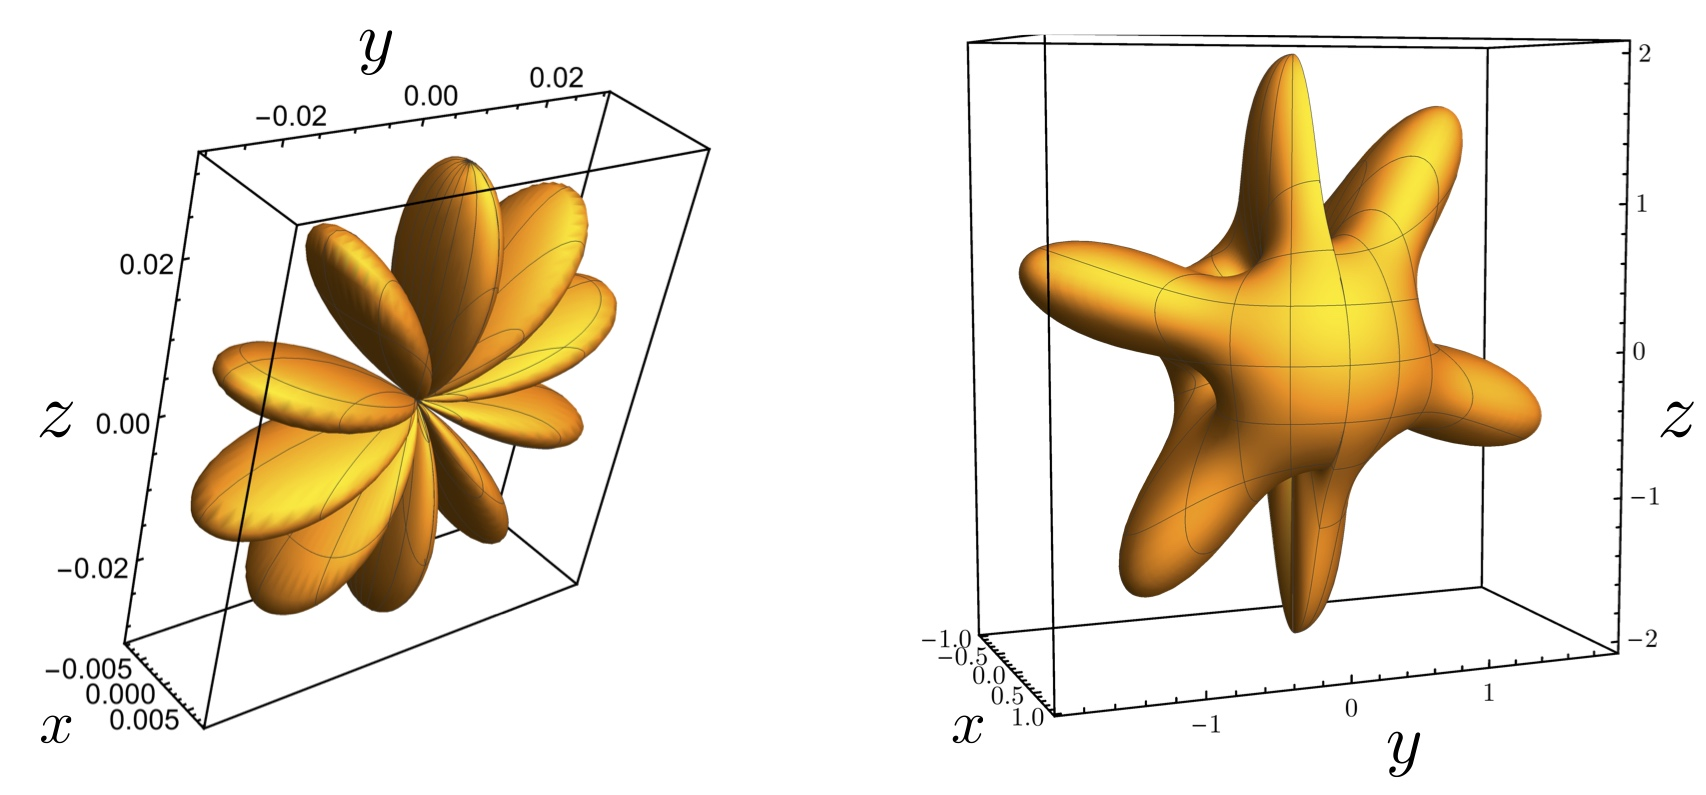
\includegraphics[width=\columnwidth]{experimentalQSE-Insieme.jpg}
    \caption{Spherical polar plot of the interference term $-\text{Re}[q_+(5/2,\alpha,\beta)q^*_-(5/2,\alpha,\beta)]$ in the $Q_2(\alpha,\beta)$ function.}
    \label{fig:expQWs:SCS_plots}
\end{figure}



\section{Conclusions}
\label{sec:expQWs:conclusions}

In this chapter we presented an experimental implementation of the state engineering protocol discussed in~\cref{chapter:quantum_walks}. We realised the QW with a photonics apparatus using \ac{OAM} and polarisation as physical embodiments of walker and coin degrees of freedom.
In particular, we implemented a five-step \ac{QW} with full control the preparation, choice of coin operations, and detection stages. To showcase the effectiveness of the protocol, we demonstrated the synthesis of arbitrary walker states.
Our results reinforce the idea that numerical optimisation complementing a complex \ac{QW} dynamics is effective for high-dimensional state engineering.
Future outlooks of this work include using our platform to implement quantum information protocols involving entanglement between low- and high-dimensional degrees of freedom, as well as exploring the possibility of achieving entanglement between the OAM of multiple photons, by leveraging the rich possibilities offered by the QW dynamics.
% A natural generalisation of this novel paradigm could be the engineering in the multipartite scenario, exploiting quantum correlations between multiple walkers. Regarding the research of the coin, further improvements of our approach can be envisaged by identifying appropriate routines to optimize the state engineering process in the presence of actual experimental imperfections.
% To this end, machine learning algorithms can be a promising add-on to our numerical optimisation approach to adapt the coin operators to a given experimental implementation.
